%%%Pregunta 1
\section{Ruteo}

Realice el ruteo del siguiente programa e indique qué es lo que imprime. Cada vez que el valor de una variable cambie, escríbalo en una nueva fila de la tabla. Recuerde que si una variable
es de tipo \textit{string}, su valor debe ir entre comillas simples ’ ’.

Importante: La tabla tiene suficientes filas.

\begin{figure}[h]
	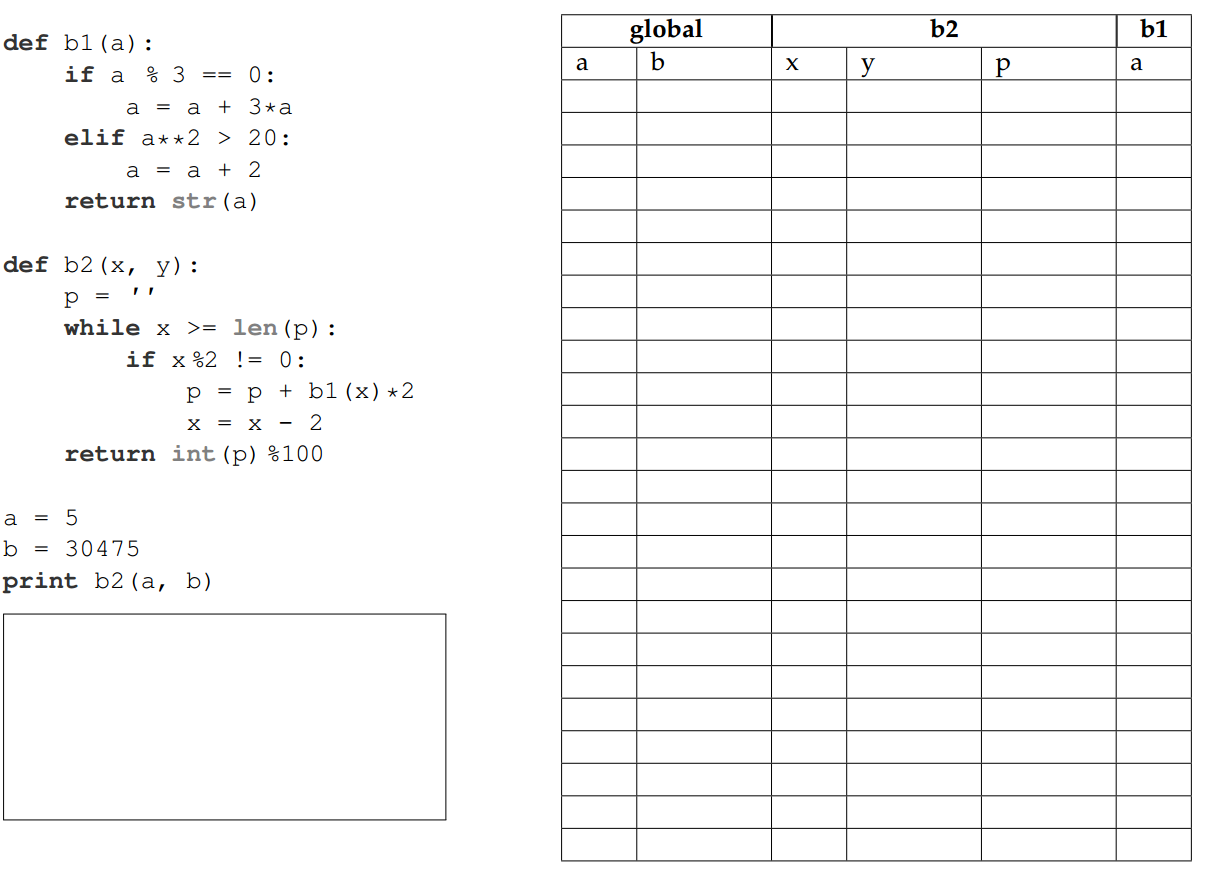
\includegraphics[scale=0.67]{Imagenes/1_c1_2015_1.png}
\end{figure}

\newpage